%!TEX root = ../main.tex
\chapter{Calorimetry and the Particle Flow Concept}
\label{chap:CaloPFA}

In high energy physics, calorimeters are fundamental tools used to measure the energy of particles. This is done by measuring signals from interactions of high energy particles with atoms in matter. This chapter will give a brief overview of the physics that describes interactions of particles with matter. The modeling of showers is discussed in chapter \ref{chap:G4Simulation}. Additionally, a brief description of the properties of calorimeters and an introduction to the \textit{Particle Flow Concept} which drives the designs of the calorimeters for ILC will be discussed.

\section{Particle interaction with matter}
\label{sec:PartInter}

In this section, a short description of the interaction of particles with matter will be given. This includes electromagnetic showers induced by electrons and photons, the energy loss by heavy charged particles and the development of hadronic showers. Moreover, the consequences of these interactions on calorimetric measurements will be discussed.

\subsection{Electromagnetic showers}
\label{subsec:EMShowers}

\subsubsection{Energy loss by electrons/positrons}

High energy electrons lose their energy via different processes depending on their kinetic energy. At low energies, below few tens of MeV, electrons (positrons) lose their energy via ionization primarily. However, more processes are contributing such as Bhabha scattering, M\o{}ller scattering. At energies above 100 MeV, the principal source of energy loss is from \textit{Brems\-strah\-lung} photons due to the Coulomb interaction of the electron in the electric field of the nuclei. The emitted photons follow an energy spectrum that falls off as $1/E$ \cite{Wigmans:392793}. The different contributions to the electron energy loss as a function of the energy are shown in figure \ref{fig:ElossEM}. The transition point where the energy losses due to ionization and Bremsstrahlung are roughly equivalent is generally referred to as the critical energy $\epsilon_{c}$. The critical energy is material dependent and for solids, it can be parametrized as
\begin{equation}
  \epsilon_{c} = \frac{\SI{610}{\mega\eV}}{(Z + 1.24)}
\end{equation}
The critical energy for iron is around \SI{21}{\mega\eV}.

\subsubsection{Energy loss by photons}

High energy photons lose their energy via \textit{pair production} where the photon creates an electron-positron pair caused by the nuclear electric field. However for this process, the photon energy needs to be at least the rest mass of the $e^+e^-$ pair ($E_{\gamma} \geq 2 \times \SI{511}{\kilo\eV}$). The photon specific cross-sections as a function of the photon energy are shown in figure \ref{fig:GammaEMloss}. For energies below the pair production threshold, it is most likely to interact via the \textit{photo-electric effect}. In this process, the photon is absorbed by the atom and an electron is emitted. The excited atom goes back to ground state by the radiation of Auger electrons or X-rays. Additional processes are contributing to the photon energy loss such as the \textit{Rayleigh} or \textit{Compton} scattering where the photon is scattered coherently or incoherently by an electron of the atom nuclei.

\begin{figure}[htbp!]
  \centering
  \begin{subfigure}[t]{0.56\textwidth}
    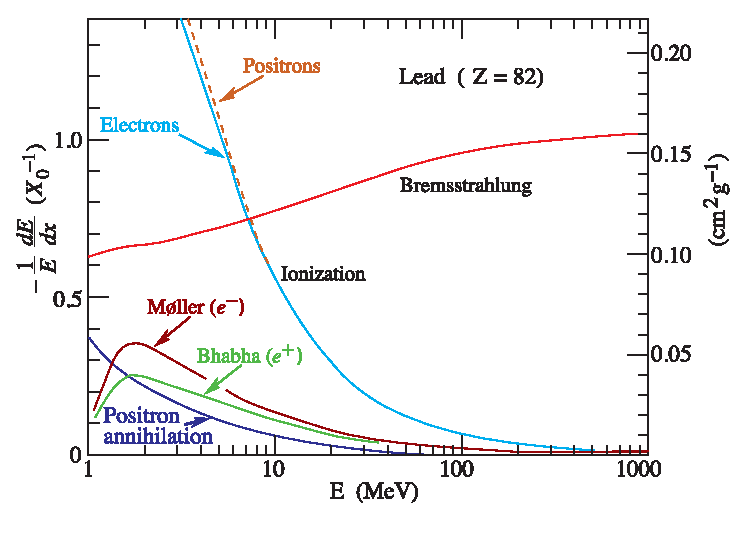
\includegraphics[width=1\linewidth]{chap2/fig/elossfrac_06.eps}
    \caption{} \label{fig:ElossEM}
  \end{subfigure}
  \hfill
  \begin{subfigure}[t]{0.43\textwidth}
    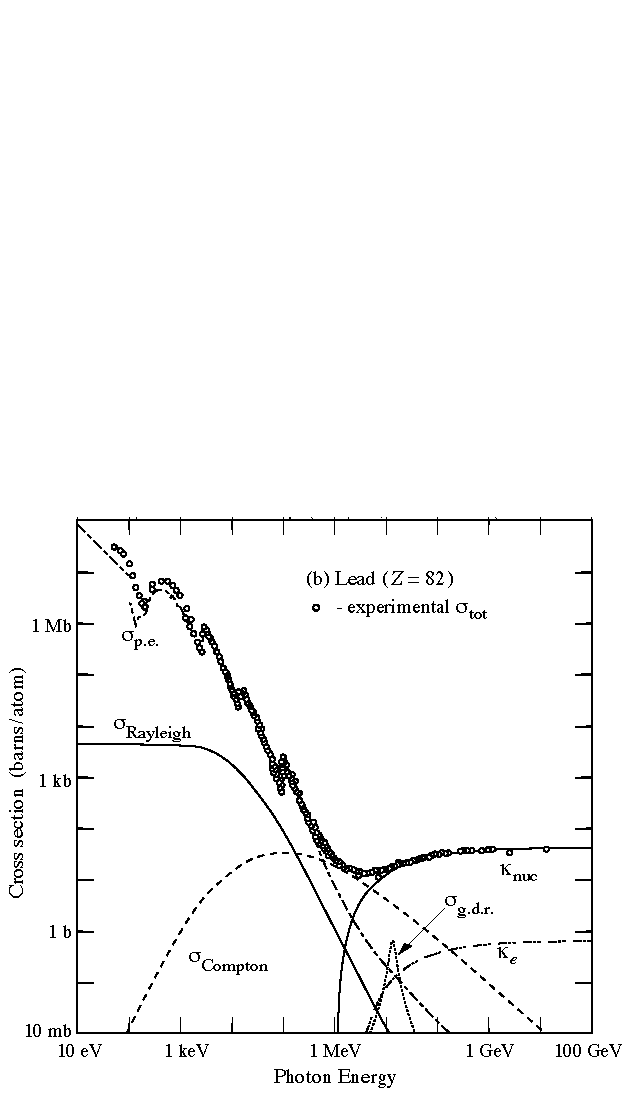
\includegraphics[width=1\linewidth]{chap2/fig/sigma_both_06.pdf}
    \caption{} \label{fig:GammaEMloss}
  \end{subfigure}
  \caption{\subref{fig:ElossEM}) Energy loss for electrons in lead as a function of the energy. All the different processes contributing to the electron energy loss are represented. \subref{fig:GammaEMloss}) Photon total cross-section as function of the photon energy in lead. $\sigma_{p.e.}$ is the photo-electric cross-section, $\sigma_{g.d.r.}$ is the photonuclear cross-section (Giant Dipole Resonance \cite{Berman:1975tt}) where the target nucleus is broken up, $\kappa_{e}$ is the pair production cross-section in an electron field and $\kappa_{nuc}$ is the pair production cross-section in a nuclear field \cite{Patrignani:2016xqp}.}
\end{figure}

\subsubsection{Electromagnetic cascades}
\label{subsubsec:EMcascade}

A cascade initiated by a multi-GeV electron involves all the processes described above. A simple model of the development of electromagnetic shower is shown in figure \ref{fig:EMDevel}. The Bremsstrahlung process plays an important role in electromagnetic cascades. A large number of photons are radiated once the electron enters matter. Most of these photons are very soft and thus will get absorbed by Compton scattering and the photo-electric effect. However, a number of photons have the necessary energy to undergo pair production. These new electrons radiate, in turn, Bremsstrahlung photons creating new branches in the cascade. This results in the multiplication of the number of particles. The number of generated particles in an electron shower of energy $E_0$ is around $N \approx \frac{E_0}{\epsilon_{c}}$.

\begin{figure}[htbp!]
  \centering
  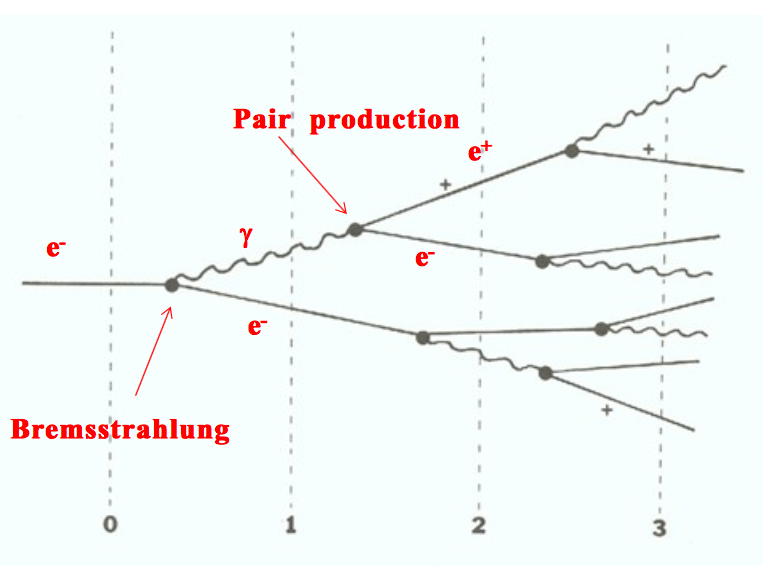
\includegraphics[width=0.6\linewidth]{chap2/fig/EM_shower_dev.png}
  \caption{Simple model illustrating the development of an electromagnetic shower. The x-axis represents the depth of the shower in radiation length $X_0$. The y-axis represents the lateral development of the shower in Moli\`ere radius $\rho_{M}$.} \label{fig:EMDevel}
\end{figure}

The development of the cascade stops when the average electron energy is around $\epsilon_{c}$. The longitudinal depth where this occurs is called the \textit{shower maximum}. The mean shower maximum $x$ is parametrized as
\begin{equation}
  \frac{x}{X_0} = \ln\left(\frac{E_0}{\epsilon_{c}}\right) + C
\end{equation}
where the constant C = -0.5 for electron induced showers and C = 0.5 for photon induced showers. Therefore it follows a logarithmic dependence on the initial electron energy \cite{Wigmans:392793}.

The longitudinal containment of the shower scales similarly with $\ln\left(E_0\right)$. On average, 95\% of the deposited energy of a 10 GeV electron is contained within 14 $X_0$ of copper, for a 1 TeV electron, around 22 $X_0$ of copper is needed \cite{Wigmans:392793}.

Typically electromagnetic showers are described by the \textit{radiation length} $X_0$ for the longitudinal development and by the \textit{Moli\`ere radius} $\rho_{M}$ for the lateral development. The radiation length is defined as the distance over which a high energy electron (positron) loses $(1 - e^{-1}) = 63.2\%$ of its initial energy by Bremsstrahlung. A common parametrization of $X_0$ as a function of the atomic number $Z$ and the atomic mass number $A$ is \cite{Wigmans:392793}
\begin{equation}
  X_0 = \frac{716 \times A}{Z(Z+1)\ln\left(287/\sqrt(Z)\right)} [\frac{g}{cm^2}]
\end{equation}
For high energy photons, the radiation length is related to the \textit{mean free path} $\lambda_{\gamma}$ of the photon, i.e the typical distance in which the photon travels before undergoing pair production as
\begin{equation}
  \lambda_{\gamma} = \frac{9}{7} X_0
\end{equation}

The lateral development of an electromagnetic shower is characterized by the Moli\`ere radius $\rho_{M}$. On average, 90\% of the energy of the shower will be contained into a cylinder of radius $\rho_{M}$. The Moli\`ere radius is parametrized as \cite{Wigmans:392793}
\begin{equation}
  \rho_{M} = \SI{21.2}{\mega\eV} \quad \frac{X_0}{\epsilon_c}
\end{equation}

\subsection{Interaction of charged heavy particles}
\label{sec:InteracHeavyPart}

As explained above Bremsstrahlung is the main process in which particles lose their energy. But this process is suppressed by the particle mass as $1/m^4$, thus for muons or charged hadrons, ionization is the main process for energy loss. The mean energy loss of a heavy charged particle is given by the Bethe-Bloch formula \cite{Wigmans:392793}
\begin{equation}
  \left<\frac{dE}{dx}\right> = Kz^2\frac{Z}{A}\frac{1}{\beta^2}\left(\frac{1}{2}\ln\frac{2m_ec^2\beta^2\gamma^2T_{max}}{I^2} - \beta^2 - \frac{\delta}{2}\right)
\end{equation}
where $T_{max}$ is the maximum single collision energy transfer, $I$ is the mean excitation energy of the absorber, $\delta$ is a correction term for then density effect depending on $\beta\gamma$, K is a constant equals to $4\pi{}N_Ar_e^2m_ec^2$, $\beta$ is the particle velocity and $\gamma$ is the Lorentz factor. The figure \ref{fig:BetheBloch} shows the mean energy loss for muons in copper as function the particle momentum and $\beta\gamma = \frac{p}{mc}$.

\begin{figure}[htbp!]
  \centering
  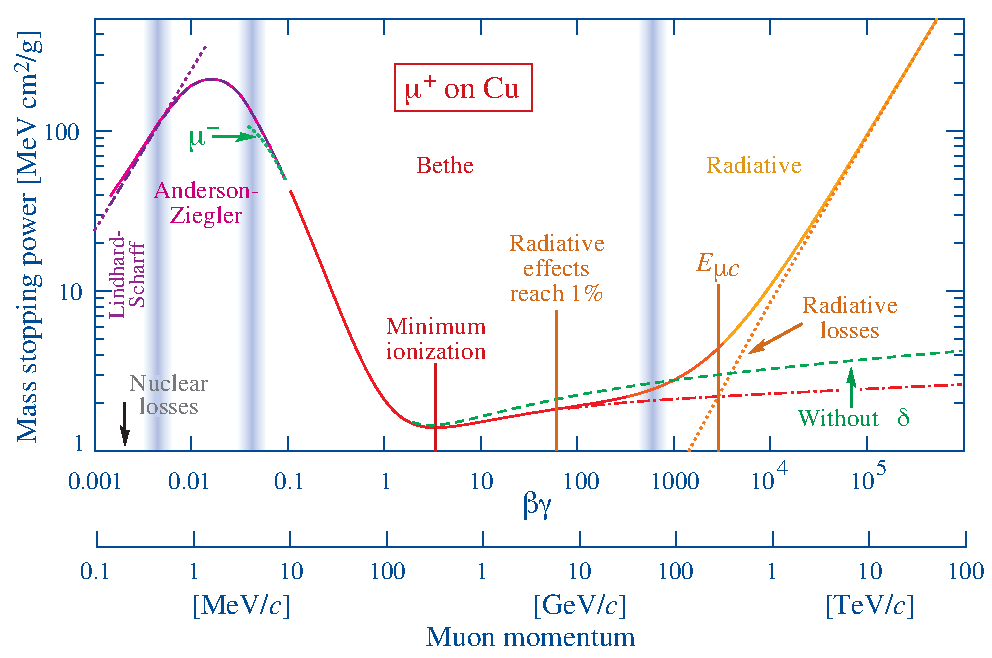
\includegraphics[width=0.6\linewidth]{chap2/fig/rpp_icru49_cu_col.pdf}
  \caption{Mean energy loss of muons in copper as a function of particle momentum. Vertical bands indicate boundaries between model transitions \cite{Patrignani:2016xqp}.} \label{fig:BetheBloch}
\end{figure}

Below 100 GeV, ionization effects dominate in the energy loss and present a broad minimum around 1 GeV ($\beta\gamma \sim 2-4$). Particles in that region are generally referred as \textit{Minimum Ionizing Particles} (\acrshort{mip}). Above 100 GeV, radiative effects become more important than ionization.

The energy loss distribution by heavy charged particles in thin materials follows a Landau distribution. However, the most probable value (MPV) for the energy deposition is below the value of the mean energy deposition $\left<\frac{dE}{dx}\right>$ by around 60\% and has a long tail toward high energy losses due to:
\begin{itemize}
  \item The production of $\delta$-electrons when a significant amount of energy is transferred in a collision
  \item Bremsstrahlung photons that can initiate small electromagnetic Showers
  \item Nuclear reactions with the nucleus of the material giving rise to high local energy deposits
\end{itemize}
The most probable value of the energy loss distribution is less dependent on the momentum of the particle than the mean energy loss $\left<\frac{dE}{dx}\right>$, therefore the most probable value can be used as a natural energy deposition scale (see chapter \ref{chap:ECalibAHCAL}).

\subsection{Hadronic showers}
\label{subsec:HadShowers}

Hadrons interact strongly such as many different processes can occur. Afterwards, the products of the interaction can again interact with the absorber material, thus leading to hadronic showers. A representation of the development of a hadronic shower is shown in figure \ref{fig:HadShower}.

Hadronic shower can be characterized by the \textit{nuclear interaction length} $\lambda_{int}$ which is defined as the mean free path travelled by a hadron before undergoing an inelastic interaction. Typically, this scale is generally much larger than $X_0$, for example, $\lambda_{int}/X_0 \sim 9.5$ in iron. This variable depends on the particle type thus also size as it depends on the inelastic cross-section. The \textit{pion interaction length} $\lambda_{\pi}$ is around 3/2 times larger than the interaction length for protons \cite{Wigmans:392793}. Similar to electromagnetic showers, the longitudinal depth of the shower increases logarithmically with the energy of the incoming hadron.

In general, hadronic shower contain two components, an electromagnetic component and a hadronic component.

\begin{figure}[htbp!]
  \centering
  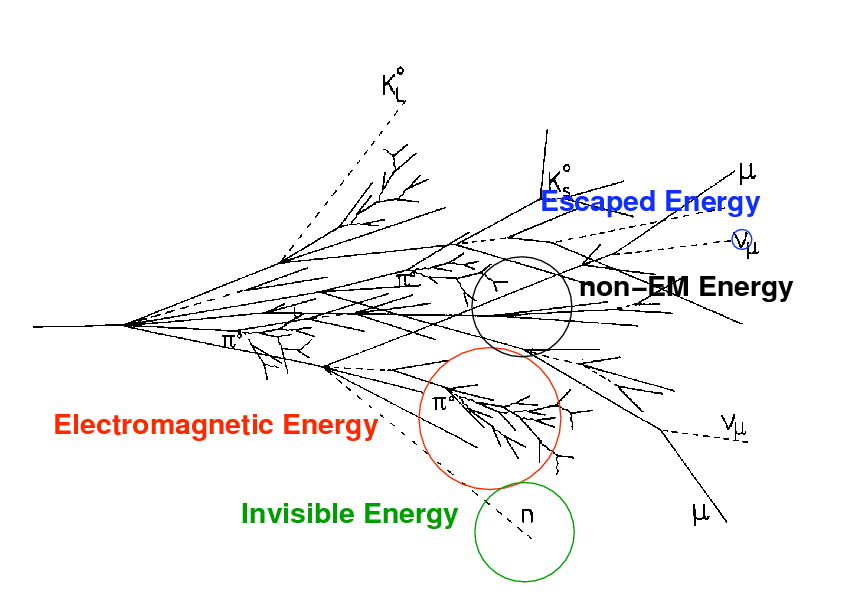
\includegraphics[width=0.6\linewidth]{chap2/fig/images_had-shower.png}
  \caption{Schematic of a hadronic shower. The different "types" of energy are represented in colors. Electromagnetic energy: decay of $\pi^0$s and $\eta$s to $\gamma$s. Non-EM energy: ionization by charged hadrons, spallation. Escaped energy: neutrinos from hadron decays. Invisible energy: nuclear binding energy, neutron scattering and capture \cite{Grahn:2009ki}.} \label{fig:HadShower}
\end{figure}

\subsubsection{Electromagnetic component}

When a hadron interacts strongly with the medium, it produces a number of secondary particles, in particular, $\pi^0$s and $\eta$s, which have a very short life ($\sim 10^{-7}$s) and decay electromagnetically to photons such as
\begin{equation*}
  \begin{aligned}
    &\pi^0 \rightarrow 2\gamma \quad (99\%)\\
    &\eta \rightarrow 2\gamma \quad (39\%)\\
    &\eta \rightarrow 3\pi^0 \quad (33\%)\\
    &\eta \rightarrow \pi^0 + 2\gamma \quad (0.03\%)
  \end{aligned}
\end{equation*}
Per hadron collision, on average, 1/3 of the available energy will be carried by the electromagnetic component. If the initial energy of the projectile is sufficient, after $n$ generations of reactions, the average electromagnetic fraction $<f_{EM}>$ can be parametrized as \cite{Wigmans:392793}
\begin{equation}
  <f_{EM}> = 1 - (1 - \frac{1}{3})^n
\end{equation}
However, this is a very simplified model and should be seen only as an upper limit due to other effects (baryon number conservation, ionization and nuclear excitations...) which lower the average electromagnetic fraction. Typically, $<f_{EM}>$ increase as a function of the initial particle energy. For example, a 10 GeV pion in copper has $<f_{EM}> = 0.38$ and at 1 TeV $<f_{EM}> = 0.73$ \cite{Wigmans:392793}. However, this is an average electromagnetic fraction, it generally varies strongly from shower to shower.

\subsubsection{Hadronic component}
\label{subsubsec:HadComp}

When a high energy hadron interacts with a nucleus, several processes are possible due to the strong interaction: \textit{spallation}, \textit{evaporation} and \textit{fission}.

Spallation is the most probable interaction. This process can be described in two stages: a fast intra-nuclear cascade involving the constituents of the nucleus and a slow nuclear evaporation. In the first stage, the incoming hadron interacts strongly with the nucleons of the nucleus producing a cascade of new stable and unstable hadrons. The resulting hadrons can then, in turn, interact with a nucleus or they can decay.

The second stage consists of the de-excitation of the nucleus by evaporating free nucleons until the excitation energy is less than the binding energy of the nucleus. This binding energy is often called \textit{invisible energy} as it is lost during the measurement process. Nevertheless, this energy can be regained by using materials with high fission cross-section such as $^{238}U$.

During spallation, plenty of neutrons can be released. These neutrons are \textit{invisible} to the calorimeter and scatter through the calorimeter (mean free path $\sim$ cm) until they lost most of their kinetic energy (\textit{thermalization}). Then these neutrons can get captured by a nucleus as the capture cross-section is maximal at rest. This process leads to late energy depositions ($\sim$ min). The excited nucleus emits $\gamma$-rays usually to get rid of the excess energy.

Since the \textit{invisible} energy only occurs in hadron showers, this leads to a difference of the calorimeter response between electrons and hadrons of the same energy. This introduces the term of \textit{compensation} that will be described in section \ref{subsec:Compensation}.

\subsubsection{Time development}
\label{sec:TimeDevShowers}

electromagnetic cascades develop at the speed of light due to the prompt generation of particles with relativistic energies. However, hadronic cascades have different components which have an impact on the time development of the shower. The electromagnetic component is prompt as an electromagnetic cascade but the hadronic component can be delayed significantly due to nuclear excited states ($\sim$\si{\micro\second}) and the release of thermal neutrons ($\sim$\si{\micro\second}-\si{\second}). Thermal neutrons can travel significantly through the detector before being captured by a nucleus and generating a signal in the calorimeter. These effects have an impact  on the reconstructed energy and spatial development of the shower due to the time acceptance of the readout electronics.

\section{Calorimeters}

Calorimeters are used to absorb an incident particle and measure the deposited energy. As explained in \ref{subsec:EMShowers} and \ref{subsec:HadShowers}, the longitudinal depth of the shower scales logarithmically with the energy of the incoming particle. Thus the energy of a shower can be mostly contained completely with a moderate amount of material, even for very high energy particles. Calorimeters can be separated in two types: \textit{homogenous} and \textit{sampling} calorimeters.

\subsubsection*{Homogenous calorimeters}

In homogenous calorimeters, the complete detector volume is sensitive to particle energy depositions. An example of homogenous calorimeter is the ECAL used by the CMS detector. It uses $PbWO_4$ scintillating crystals of around $2.2 \times 2.2 \times 23$ cm$^3$, these have very short radiation length ($X_0$ = 0.85 cm) and Moli\'ere Radius ($\rho_M$ = 2.19 cm) allowing for a compact design. As this calorimeter is homogenous, the entire kinetic energy of an incoming electron or photon can be measured, reducing sampling fluctuations and achieving a very good single particle energy resolution\footnote{Explained in \ref{subsec:EnergyReso}.} of $\sigma_E/E \approx 2.8\%/\sqrt(E) \oplus 0.3\%$ \cite{1742-6596-587-1-012001}.

\subsubsection*{Sampling calorimeters}

In sampling calorimeters, the calorimeter is divided into a passive medium, the absorber that is made usually of a high-density material, and an active medium that generates the signal to be measured. Sampling calorimeters offer the freedom to chose both the absorber and active material. The absorber can be chosen to minimize the amount of material while still containing most of the energy of the shower. Active materials can be chosen for special purposes, e.g an organic material with high hydrogen content to recover a part of the \textit{invisible energy} by absorbing more neutrons. Also, this allows for optimization of the design and cost. Nevertheless, it has the disadvantage of worse energy resolution than homogenous calorimeters due to sampling fluctuations as only a fraction of the energy of a shower is measured.

A sampling calorimeter can be characterized by its sampling fraction $f_{samp}$ as
\begin{equation}
  f_{samp} = \frac{E_{MIP}^{active}}{E_{MIP}^{active} + E_{MIP}^{passive}}
\end{equation}

Usually calorimeters are segmented longitudinally and laterally into small cells in order to provide information about the particle position. An electromagnetic calorimeter (ECAL) is measuring the energy of particles that interact primarily via the electromagnetic interaction, while hadronic calorimeters (HCAL) are designed to measure the energy of particles that interact strongly.

An example of a sampling calorimeter is the HCAL barrel (TileCal) in the ATLAS detector. It consists of iron plates 14 mm thick as absorber and scintillator tiles 3 mm thick as active material. The total depth of the barrel corresponds to 9.7 nuclear interaction length. It is segmented in $\phi$ and $\eta$ to provide accurate position measurement. The tiles are coupled to a wavelength shifting fiber that guides the light to two different photomultiplier tubes providing redundancy. It is the central detector for the measurements of single hadrons, jets and missing transverse energy. An energy resolution of $\sigma_E/E \approx 52\%/\sqrt(E) \oplus 3\%$ was achieved for single pions \cite{Henriques:2015fso}. This is significantly worse compared to the CMS ECAL due to the sampling fluctuations and as well due to the intrinsic fluctuations of hadron showers.

\subsection{Energy resolution}
\label{subsec:EnergyReso}

The figure of merit of every calorimeter is the energy resolution. For most calorimeters, the energy resolution $\sigma_E/E$ can be parametrized as:
\begin{equation} \label{eq:EnergyReso}
  \frac{\sigma_E}{E} = \frac{a}{\sqrt(E)} \oplus b \oplus \frac{c}{E}
\end{equation}

The first term $\frac{a}{\sqrt(E)}$ is the stochastic term. Assuming that $N$ particles contributed to the signal, the uncertainty follows a Poisson statistic such as $\sigma_N/N = \sqrt{N}/N = 1/\sqrt{N}$. Thus the stochastic term for the energy resolution follow this. Additionally, the sampling fraction $f_{samp}$ adds an additional uncertainty proportional to $\sqrt{1/f_{samp}}$. For hadronic showers, the fluctuations in the invisible energy also scales as $1/\sqrt(E)$ and the fluctuations in the electromagnetic fraction scales as $1/E^j$ with $j \leq 0.5$. For electromagnetic calorimeter, the stochastic contribution is in the order of few percent for homogenous up to around $10\%/\sqrt(E)$ for sampling calorimeters. Typically, the contribution for hadronic calorimeters is in the order of $60\%/\sqrt(E)$.

The second term $b$ is the constant term. This term is affected by detector inhomogeneities such as calibration uncertainties. This term dominates at high energies and is typically in the order of few percent.

The third term $\frac{c}{E}$ is the noise term. It is energy independent and arises from different effects like the readout electronics. This term dominates at low energies.

\subsection{Compensation}
\label{subsec:Compensation}

Due to the invisible energy fraction of a hadron shower, the calorimeter response of a hadron shower of a given energy is typically lower than the calorimeter response of an electromagnetic shower of the same energy. Calorimeters with a response ratio $e/h > 1$ are called \textit{under-compensating} while calorimeters with a response ratio $e/h < 1$ are called \textit{over-compensating}. The $e/h$ ratio decreases with energy due to the electromagnetic fraction increasing with energy.

Homogenous calorimeters have generally a significantly higher ratio $e/h \sim 2$. Sampling calorimeters can be designed to reach compensation ($e/h = 1$). To achieve compensation, either the electromagnetic response can be lowered or the hadronic response can be boosted. A famous example is the ZEUS calorimeter that used uranium (Z = 92) absorbers and plastic scintillator as active material. The thicknesses of the absorber and active material were carefully optimized to reach compensation. In this way, an energy resolution for pions of $\sigma_E/E = 35\%/\sqrt(E) + 2\%$ was achieved with $e/h \sim 1$ \cite{BERNSTEIN199323}.

Other methods can be used to achieve compensation:
\begin{itemize}
  \item \textit{Dual readout} using Cherenkov radiation to estimate the electromagnetic fraction of each event \cite{Akchurin:2013yaa}.
  \item \textit{Spacial resolution} in order to identify electromagnetic sub-showers within a hadronic shower and re-weight the whole shower or individual hits of the shower. This has been demonstrated for the H1 experiment which is using the local hit energy density to distinguish electromagnetic sub-showers from hadronic shower depositions \cite{Schacht:1990zw}.
\end{itemize}

\section{The Particle Flow approach}
\label{sec:PFA}

Calorimeters are used to measure the energy of single particles and jets. Classically, the energy is reconstructed by summing up all the energy deposits in the electromagnetic and hadronic calorimeters. In this way, typically the stochastic term from equation \ref{eq:EnergyReso} for jets is in the order of $60-100\%\sqrt{E}$. This jet energy resolution is far beyond the requirements of the ILC physics program (see chapter \ref{chap:FutureColliders}). A new approach has been developed to solve this issue and its concept is presented in this section.

\subsection{The Particle Flow concept}

Particle Flow is a new approach to calorimetry in order to achieve a jet energy resolution much better than traditional calorimetry approaches (order of twice better). \textit{Particle Flow Algorithms} (\acrshort{pfa}) aim to reconstruct the energy of all the individual contributions inside a jet. This was made possible by the significant improvements in tracking detectors and calorimeters over the last decade. A schematic of the Particle Flow concept is shown in figure \ref{fig:PFAConcept}.

\begin{figure}[htbp!]
  \centering
  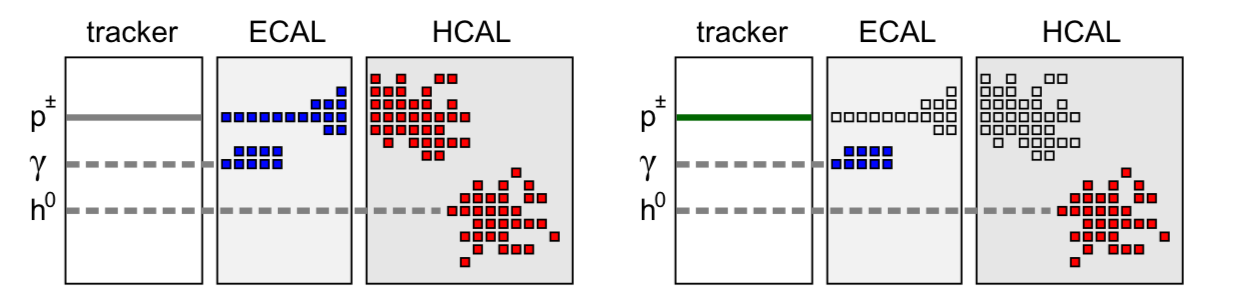
\includegraphics[width=1\linewidth]{chap2/fig/PFAConcept.png}
  \caption{Schematic of the Particle Flow Concept. On the left: Traditional calorimetry, The ECAL and HCAL measure the energy deposited by all particles in a jet (charged particles, photons and neutral particles). The tracker information is not used. On the right: Particle flow approach, The tracker measures all charged particles and the calorimeter information is removed, the ECAL measures the photons and the HCAL measures only neutral particles \cite{Feege:2011dsa}.} \label{fig:PFAConcept}
\end{figure}

On average in a jet, 60\% of the energy is carried by charged hadrons, 30\% by photons and 10\% by neutral hadrons \cite{Ebrahimi:394104}. As hadronic calorimeters have a poor energy resolution ($\sim 60\%/\sqrt{E}$), by a pure calorimetric approach, 70\% of the energy would be poorly measured. Therefore, the poor resolution of the HCAL is dominant in the jet energy resolution.

The Particle Flow reconstruction requires an unprecedented longitudinal and lateral segmentations for the calorimeters in order to distinguish depositions of charged and neutral particles in the calorimeter as well as an excellent tracking system. This approach uses the best sub-detector measurement for each particle in a jet. All charged particle are measured by the tracker due to the excellent tracker resolution, photons are measured in the ECAL and neutral hadrons are measured in the HCAL. In this case, only around 10\% of the energy is measured poorly by the HCAL and thus its impact on the jet energy resolution is lessened.

The Particle flow approach at the ILC has the potential to improve the jet energy resolution to around 3-4\% in the range of 45 to 250 GeV ($\sim 30\%/\sqrt{E}$). The jet energy resolution can be parametrized as
\begin{equation}
  \sigma_{jet} = f_{charged} \cdot \sigma_{Tracker} \oplus f_{\gamma} \cdot \sigma_{ECAL} \oplus f_{neutral} \cdot \sigma_{HCAL} \oplus \sigma_{conf} \oplus \sigma_{leak}
\end{equation}
$\sigma_{Tracker}, \sigma_{ECAL}, \sigma_{HCAL}$ are the energy resolutions of the tracker, ECAL and HCAL respectively, contributing to the jet energy resolution with weighted fractions of the particle type in the event.

$\sigma_{conf}$ represents the confusion term due to the possibility of wrong assignments of tracks and calorimeter energy depositions. There are three main sources of confusion:

\begin{itemize}
  \item A part (or all) of the shower from a charged hadron is reconstructed as a neutral cluster. This lead to the double-counting of energy.
  \item A part (or all) of a neutral shower is associated to a charged shower. This lead to the lost of the energy of the neutral particle, therefore, energy is missing.
  \item The failure to resolve photons close to a charged hadron track leading to the loss of the photon energy.
\end{itemize}

The confusion is a limiting factor in Particle Flow calorimetry and starts to dominate for high jet energies. Other contributions are present such as $\sigma_{leak}$ that degrade the jet energy resolution due to leakage in the calorimeter and uninstrumented areas.

\subsection{Implementation in PandoraPFA}

Some implementations of PFAs were made in the past like H1 at HERA \cite{Abt:1994ye} and up to now in CMS at the LHC \cite{Sirunyan:2017ulk}. However, these detectors were not designed and optimized for particle flow reconstruction. The ILC detectors are designed in such a way that they offer the best instrumentation for the application of the particle flow concept.

PandoraPFA \cite{Thomson:2009rp, Marshall2013} is an implementation of the Particle Flow Concept for the ILC. It reconstructs individual particles using the information provided by the highly granular calorimeters and the tracker. The algorithm operates in several stages:
\begin{itemize}
  \item Tracks are categorized based on topology. Kinks, V0s from neutral particle decays, e.g $K_s \rightarrow \pi^+\pi^-$, are identified and treated separately by the algorithm.
  \item Calorimeter hits are clustered using a simple cone-based algorithm starting at the front face of the ECAL going to the back of the HCAL. Tracks seeds from the projection of tracks to the front face of the ECAL can be used for the cluster starting point. The clustering algorithm is configured in a way that it tends to split more the energy deposits than accidentally merging particles in this early stage. The clustering follows certain topological rules and exploit the spatial resolution of the calorimeters to minimize clustering mistakes.
  \item The calorimeter clusters are associated to tracks. The algorithm compares the cluster energy and track momentum and other properties such as the track direction at the front face of the ECAL and cluster orientation to make the correct associations.
  \item If the energy of a cluster and the associated momentum of a track don't agree, a statistical re-clustering is performed using different parameters until a better track-cluster compatibility is found.
  \item The algorithm identify photons based on shower profile information in order to recover photons that are merged with a charged hadron shower.
  \item Fragments of hadron showers are identified and the algorithm looks for neutral fragments that are mis-identified coming from nearby charged clusters. These fragments are merged into the parent charged cluster and the track-cluster compatibility is evaluated again.
  \item A Particle Flow Object (PFO) is constructed. Track properties are used for charged particles, the calorimeter information is used for neutral particles.
\end{itemize}
The details of theses stages and possible other stages are described in more details in \cite{Thomson:2009rp}.

\begin{figure}[htbp!]
  \centering
  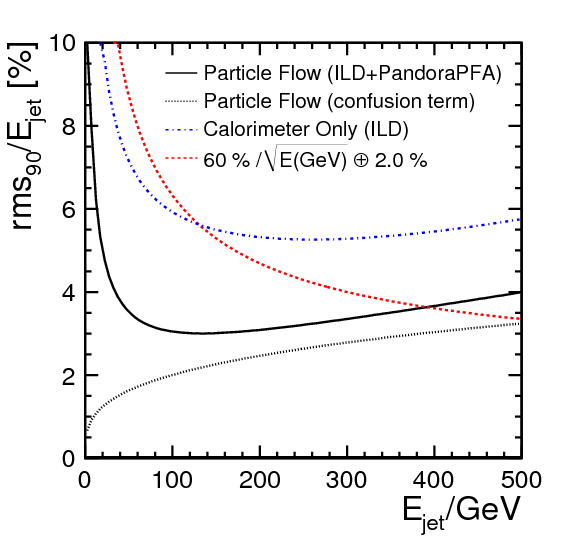
\includegraphics[width=0.6\linewidth]{chap2/fig/pfa_figure_10.png}
  \caption{Empirical jet energy resolution as function of the jet energy for PandoraPFA and the ILD detector. The estimated contribution of confusion is represented by the back dotted line. The dotted-dashed blue curve shows the jet energy resolution only from the calorimetric depositions. Moreover, a parametrization of a typical jet energy resolution ($\frac{60\%}{\sqrt{E}} \oplus 2\%$) is shown in red using the traditional calorimetry approach \cite{Thomson:2009rp}.} \label{fig:ILDPFA}
\end{figure}

The jet energy resolution obtained in ILD with Pandora PFA is shown in figure \ref{fig:ILDPFA}. The figure shows that the jet resolution obtained is much better than in traditional calorimetry. It also shows that the goal of 3-4\% relative jet energy resolution is achieved over a large jet energy range.

\begin{center}
  \rule{0.5\textwidth}{.4pt}
\end{center}

As shown in this chapter, jet energy measurements with an excellent resolution can be achieved with the particle flow approach. This approach requires an excellent tracker and highly granular calorimeters. The development of such calorimeters is discussed in the following chapter.
